
\chapter{Weiner's Approach}











\section{Finding the Jamming Limit}

We first look at Weiner's elementary approach to finding the jamming limit $C_R$ 
(see \cite{weiner1969elementary}). Using our previously derived master equation 
(\ref{eq:3}) Weiner solved for $M(x)$ recursively, giving us the following 
results: \bigskip

\begin{eqnarray} \label{eq:4}
	M(x) = 
	\begin{dcases}
		0                                   & \text{if } x \in [0, 1) \\\\
		1                                   & \text{if } x \in [1, 2) \\\\
		3 - \frac{2}{x - 1}                 & \text{if } x \in [2, 3) \\\\
		7 - \frac{10 - 4 \ln(x - 2)}{x - 1} & \text{if } x \in [3, 4)
	\end{dcases}
\end{eqnarray}\medskip

\begin{table}[t!]
	\centering
	\begin{tabular}{|c | c|} 
		\hline
		$x$ & $M(x) / x$ \\ [1ex] 
		\hline
		0.99 & 0 \\ 
		1.99 & 0.5025125628 \\ 
		2.99 & 0.6672156769 \\ 
		3.99 & 0.6854478541 \\ 
		4.99 & 0.6969110964 \\ 
		5.99 & 0.7054612992 \\ 
		6.99 & 0.7114892709 \\  
		\hline
	\end{tabular}
	\caption{$M(x) / x$}
	\label{table:1}
\end{table}\medskip

and so on - the calculations becoming increasingly difficult, and frankly tedious, after this point. In 
table \ref{table:1} we have calculated $M(x) / x$ for values of $x$ close to the upper limit of each interval. 
As can be seen, the values of $M(x) / x$ seem to be approaching a limit. This can be seen more clearly in 
figure \ref{fig:rpc1}. \bigskip

\begin{figure}[h!]
	\centering
	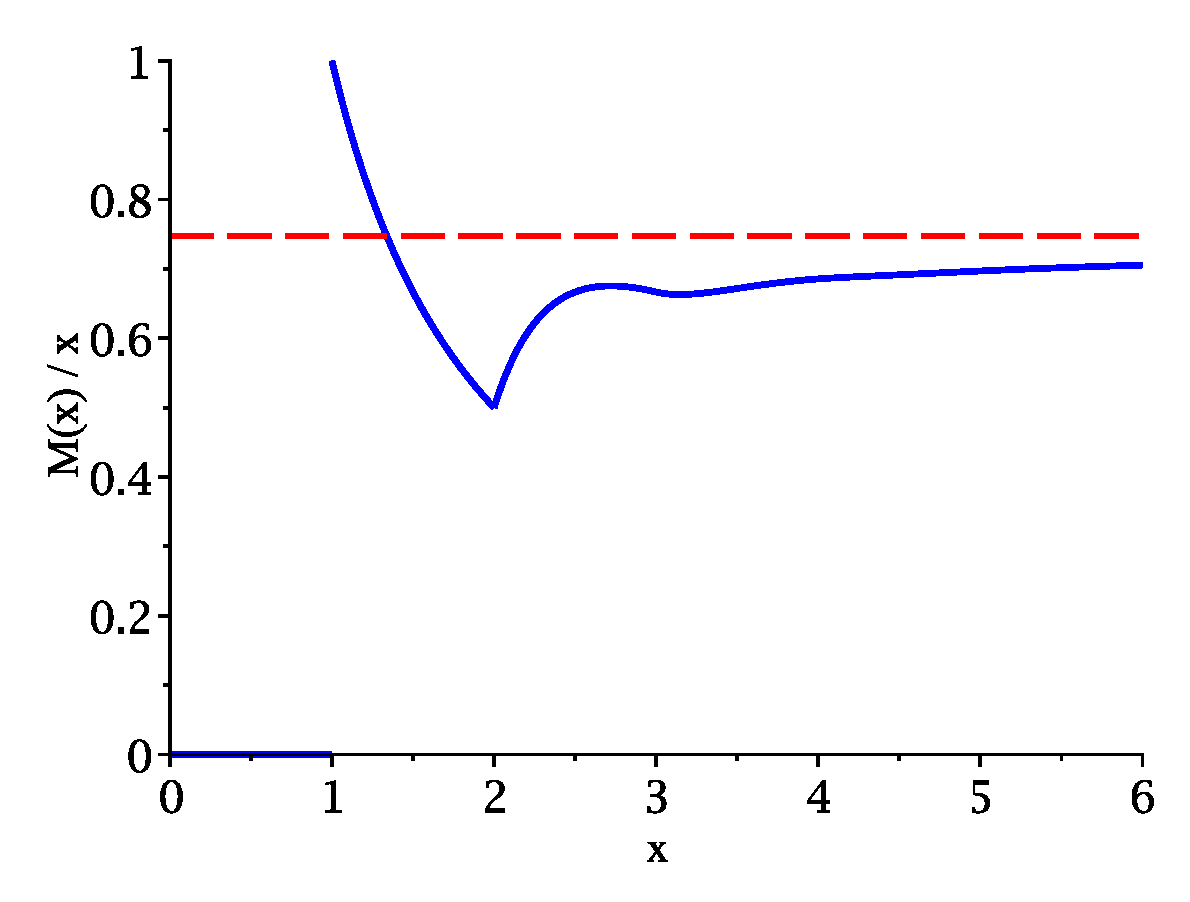
\includegraphics[scale = 0.35]{renyi_01.eps}
	\caption{R\'enyi's parking constant}
	\label{fig:rpc1}
\end{figure}\medskip











\section{Existence of the Jamming Limit}

In attempting to show that this jamming limit exists, Weiner took a flawed approach. In order to understand 
the flaw we trace his steps and return to equation \ref{eq:1}. Dividing across by $x$ we get: \bigskip

\begin{eqnarray} \label{eq:5}
	\frac{M(x + 1)}{x} = \frac{1}{x} + \frac{2}{x^2} \int_{0}^{x} M(t) dt
\end{eqnarray}\medskip

differentiating with respect to $x$: \bigskip

\begin{eqnarray*}
	\left(\frac{M(x + 1)}{x}\right)^{\prime} = -\frac{1}{x^2} - \frac{4}{x^3} \int_{0}^{x} M(t) dt + \frac{2}{x^2} M(x)
\end{eqnarray*}\medskip

looking at the integral, and making use of the fact that $0 \leq M(x) \leq x$ we find that: \bigskip

\begin{eqnarray*} 
	\int_{0}^{x} M(t) dt & \leq & \int_{0}^{x} t dt \\\\
						 & \leq & \frac{x^2}{2}
\end{eqnarray*}\medskip

making use of both we find: \bigskip

\begin{eqnarray*} 
	\left(\frac{M(x + 1)}{x}\right)^{\prime} & =    & -\frac{1}{x^2} - \frac{4}{x^3} \int_{0}^{x} M(t) dt + \frac{2}{x^2} M(x) \\\\
											 & \leq & -\frac{1}{x^2} - \frac{4}{x^3} \cdot \frac{x^2}{2} + \frac{2}{x^2} \cdot x \\\\
											 & \leq & -\frac{1}{x^2} - \frac{2}{x} + \frac{2}{x} \\\\
											 & \leq & -\frac{1}{x^2} \\\\
											 & =    & \mathcal{O}\left(\frac{1}{x^2}\right) 
\end{eqnarray*}\medskip

and hence: \bigskip

\[
	\lim_{x \to \infty} \left(\frac{M(x + 1)}{x}\right)^{\prime} = 0
\]\medskip

which according to Weiner implies that: \bigskip

\[
	\lim_{x \to \infty} \frac{M(x)}{x} = C_R
\]\medskip

this, however, is incorrect, as a simple counterexample will demonstrate. We consider: \bigskip

\begin{eqnarray*}
								 f(x) & = & \sin(\ln(x)) \\\\
						f^{\prime}(x) & = & \frac{\cos(\ln(x))}{x} \\\\
	\lim_{x \to \infty} f^{\prime}(x) & = & \lim_{x \to \infty} \frac{\cos(\ln(x))}{x} \\\\
									  & = & 0
\end{eqnarray*}\medskip

but clearly: \bigskip

\begin{eqnarray*}
	\lim_{x \to \infty} \sin(\ln(x)) & =    & [-1, 1] \\\\
									 & \neq & \text{a constant} 
\end{eqnarray*}\medskip

so this is an unsatisfactory justification for the existence of the limit. Of course if his approach 
had been to show that: \bigskip 

\[
	\left( \lim_{x \to \infty} \frac{M(x + 1)}{x}\right)^{\prime} = 0
\]\medskip

his conclusions would have been correct. However, the limit of the derivative of a function is not always 
the same as the derivative of the limit of a function. As both derivatives (and integrals) are themselves 
limits, the issue here is if the respective limits are independent. As both the limit, and the integration, 
are over $x$, then this presents a problem. \bigskip











\section{Bounds for the Jamming Limit}

Weiner did not calculate the limit, but instead provided a method for finding increasingly narrower bounds 
for the limit. Let us assume for now that: \bigskip

\[
	\lim_{x \to \infty} \frac{M(x)}{x} = C_R
\]\medskip

in order to find bounds for $C_R$ Weiner sought to sandwich $M(x)$ between two linear functions: \bigskip

\begin{eqnarray} \label{eq:6}
	L_{a_1}(x) \leq M(x) \leq L_{a_2}(x)
\end{eqnarray}\medskip

and find the limits of each of these linear functions as $x \to \infty$. Weiner found an initial lower bound 
by finding, for $x \geq 1$, the linear function of the form $L(x) = ax + b$ that satisfied the following 
equation: \bigskip

\begin{eqnarray*}
		L(x + 1) & = & 1 + \frac{2}{x} \int_{1}^{x} L(t) dt \\\\
	ax + (a + b) & = & 1 + \frac{2}{x} \int_{1}^{x} (at + b) dt \\\\
	ax + (a + b) & = & 1 + \frac{2}{x} \left[ \frac{at^2}{2} + bt \right]_{t = 1}^{x} \\\\
	ax + (a + b) & = & 1 + ax + 2b - \frac{a + 2b}{x} \\\\
		 (a + b) & = & 1 + 2b - \frac{a + 2b}{x} \\\\
		(a + b)x & = & x + 2bx - ( a + 2b ) \\\\
	(b - a + 1)x & = & a + 2b 
\end{eqnarray*}\medskip

noting that both sides of the equation must equal $0$, we arrive at two simultaneous equations: \bigskip

\begin{eqnarray*}
	 a - b & = & 1 \\
	a + 2b & = & 0
\end{eqnarray*}\medskip

from which we find the coefficients of our required linear function: \bigskip

\[
	L(x) = \frac{2}{3}x - \frac{1}{3}
\]\medskip

We know that: \bigskip

\[
	L(x) \leq M(x) = 1 \quad \text{for } 1 \leq x < 2
\]\medskip

as $M(x)$ is increasing, we see that, for $x \geq 1$: \bigskip

\[
	\frac{L(x)}{x} \leq \frac{M(x)}{x} 
\]\medskip

and hence: \bigskip

\[
	\lim_{x \to \infty} \frac{L(x)}{x} \leq \lim_{x \to \infty} \frac{M(x)}{x} 
\]\medskip

which gives us: \bigskip

\[
	\frac{2}{3} \leq C_R
\]\medskip

Weiner went on to find two linear functions that sandwiched $M(x)$ with a little more accuracy. The two 
functions found were: \bigskip

\begin{eqnarray*}
	L_{a_1}(x) & \equiv & 0.7432x - 0.2568 \\
	L_{a_2}(x) & \equiv & 0.75x - 0.25
\end{eqnarray*}\medskip

with the property found in equation \ref{eq:6} : \bigskip

\[
	0.7432x - 0.2568 \leq M(x) \leq 0.75x - 0.25 
\]\medskip

dividing across by $x$ and taking the limit as $x \to \infty$: \bigskip

\[
	0.7432 \leq C_R \leq 0.75 
\]\medskip

which gives a reasonably good indication of the bounds of $C_R$. \bigskip

%\newpage












\section{Remarks}

Weiner made use of the following theorem and lemma (both stated without proof): \bigskip

\begin{mdframed}
	\begin{theorem}
		Define $L_{a}(x) \equiv ax + a - 1$. If for some $t > 0$, $L_{a}(x) \leq M(x)$ $(L_{a}(x) \geq M(x))$ 
		for $t \leq x \leq t + 1$, then $L_{a}(x) \leq M(x)$ $(L_{a}(x) \geq M(x))$ for all $x \geq t$ \bigskip
	\end{theorem} 
	\begin{lemma}
		$M^{\prime}(x) > 0$ for $x \geq 2$ \bigskip
	\end{lemma}
\end{mdframed} \bigskip

to justify his result. \bigskip

While Weiner's approach is interesting from the point of view of it's elementary nature, it is not a 
particularly satisfying approach due to the error made in his justification of the existence of the 
limit, and also because of the "trial-and-error method" used to find the bounds. \bigskip

But while his assumption about the existence of the limit is flawed, he does provide an interesting, 
albeit dated, approach to finding the limit. His work has little more than novelty value, and is 
included in the survey because of it's historical interest - to see how the understanding of the 
problem has progressed. \bigskip











